\documentclass{VUMIFPSkursinis}
\usepackage{algorithmicx}
\usepackage{algorithm}
\usepackage{algpseudocode}
\usepackage{amsfonts}
\usepackage{amsmath}
\usepackage{bm}
\usepackage{caption}
\usepackage{color}
\usepackage{float}
\usepackage{graphicx}
\usepackage{listings}
\usepackage{subfig}
\usepackage{wrapfig}

% Titulinio aprašas
\university{Vilniaus universitetas}
\faculty{Matematikos ir informatikos fakultetas}
\department{Programų sistemų katedra}
\papertype{Programų kūrimo proceso laboratorinis darbas}
\title{Įmonės ,,Mėnuliukų technologijos" programų kūrimo proceso aprašas (Pirmas laboratorinis darbas)}
\titleineng{Description of the development process of the ,,Moon technologies" company (First laboratory work)}
\status{4 kurso 3 grupės studentai}
\author{Matas Savickis, Justas Tvarijonas, Džiugas Mažulis}
\secondauthor{Greta Pyrantaitė, Andrius Bentkus}


\supervisor{Saulius Ragaišis, Doc., Dr.}
\date{Vilnius – \the\year}

% Nustatymai
% \setmainfont{Palemonas}   % Pakeisti teksto šriftą į Palemonas (turi būti įdiegtas sistemoje)
\bibliography{bibliografija}

\begin{document}
\maketitle

\tableofcontents

\sectionnonum{Įvadas}
	Šiame darbe bus pristatyta ,,Mėnuliukai technologies" programų kūrimo procesas.
	Pats procesas yra paremtas Agile metodologija su minimaliais pakeitimais reikalavimų rinkime.
	Kūrimo procesas yra labiau pritaikytas dirbti su projektais, kurių pradžioje reikalinga surinkti daugiau informacijos ir tūrėti aiškesnį kryptį, kas bus toliau. Procesas gali vykti dviem būdais:
	\begin{itemize}
		\item{Klientas perka sistemą, kuri turės atitinkamus funkcionalumus - projekto pradžioje yra išsiaiškinama koks funkcionalumas turi būti sistemoje}
		\item{
			Klientas perka sistemos tobulinimo valandas - projekto pradžioje klientas pateikia funkcionalumų, kuriuos jis nori tūrėti sąrašą prioriteto tvarka.
			Klientas nusiperka tam tikrą skaičių darbo valandų ir tuomet laikui bėgant programuotų komanda įvertina kiek užtruks tam tikro funkcionalumo įgyvendinimas.
			Pasibaigus nusipirktom valandom nauji pakeitimai nebetiekiami kol klientas nenusiperka papildomų darbo valandų.
		}
\end{itemize}
\section{Kūrimo procesas}

	\begin{figure}[H]
	\centering
	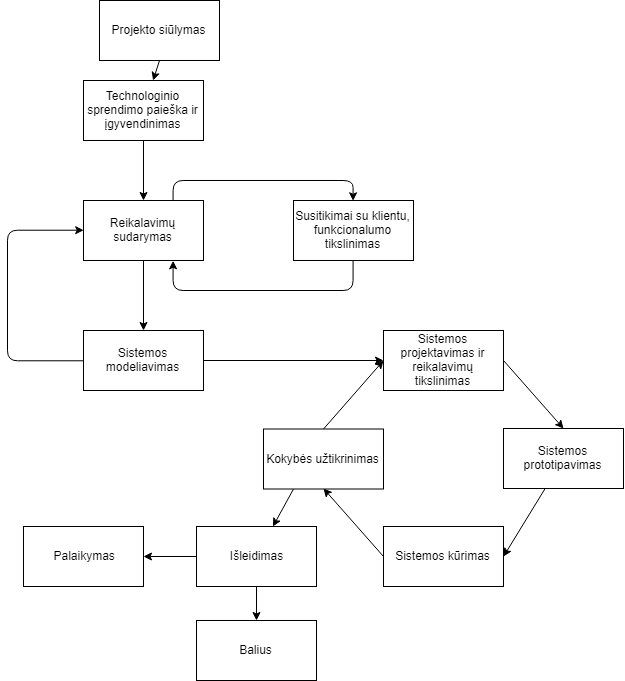
\includegraphics[scale=0.7]{img/SoftwareProcessMoonTechnologies}
	\caption{Sistemos kūrimo procesas} % Antraštė įterpiama po paveikslėlio
	\label{img:mlp}
	\end{figure}

	\subsection{Projekto siūlymas}
		Tai yra pradinė projekto fazė, kurioje yra užmezgamas dialogas su klientų. Per viešuosius pirkimus arba pačiam klientui susisiekus su įmone prasideda abstrakti sistemos analizė ir pasiūlymo sudarymas. Abstrakčioje sistemos analizėje įvertinami pagrindiniai kliento poreikiai, buvusių projektų patirtis, projekto kompleksiškumas ir dabartinė įmonės būsena. Įvertinama ar įmonė turi visus reikiamus specialistus atlikti darbui, kiek žmonių jau yra įmonėje, kiek reiktų pasisamdyti arba kokius dabus perduoti sub-kontraktoriams.
	\subsection{Technologinio sprendimo paieška ir įgyvendinimas}
		Pasirašius sutartį su klientu pradedama ieškoti konkretaus technologinio sprendimo tinkako projekto vystimui. Sutatomos konrečios karkasų, duomenų bazių arba betkokios kitos technologijos versijos kurios bus naudojamos. Jeigu projektas yra jau egzistuojantis ir klientas perka tolimesnį projekto vystimą yra išsiaiškinama ar nereikės pakelti projekte naudojamų technologijų versijos.
	\subsection{Reikalavimų ciklas}
		Nutarus dėl konkrečių technologijų, kurios bus naudojamos pradedame funkcinių ir nefunkcinių reikalavimų sudarymas. Jų sudarymas vyksta cikliškai, pirma mūsų įmonės verslo analitikas išanalizuoja verslo poreikius ir kartu su architektu sudaro pirminius reikalavimus, jie yra pristatomi klientui kartu su klausimais, įvyksta suformuotų reikalavimų aptarimas. Aptarime dalyvauja architektas, verslo analistas ir verslo žmogus. Jeigu klientas sutinka su sudarytais reikalavimais pradedamas sistemos modeliavimas, jeigu kyla neaiškumų dėl reikalavimų tarp kliento ir mūsų įmonės grįštama prie poreikių sudarimo įmonės viduje. Ciklas vyksta iki tol kol pasiekiamas sutarimas tarp mūsų įmonės ir kliento.
	\subsection{Sistemos modeliavimas}
	\begin{figure}[H]
	\centering
	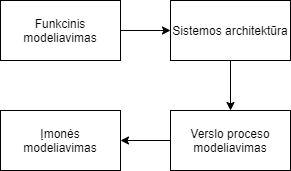
\includegraphics[scale=0.7]{img/SistemosModeliavimas}
	\caption{Sistemos modeliavimas} % Antraštė įterpiama po paveikslėlio
	\label{img:mlp}
	\end{figure}

	\begin{figure}[H]
	\centering
	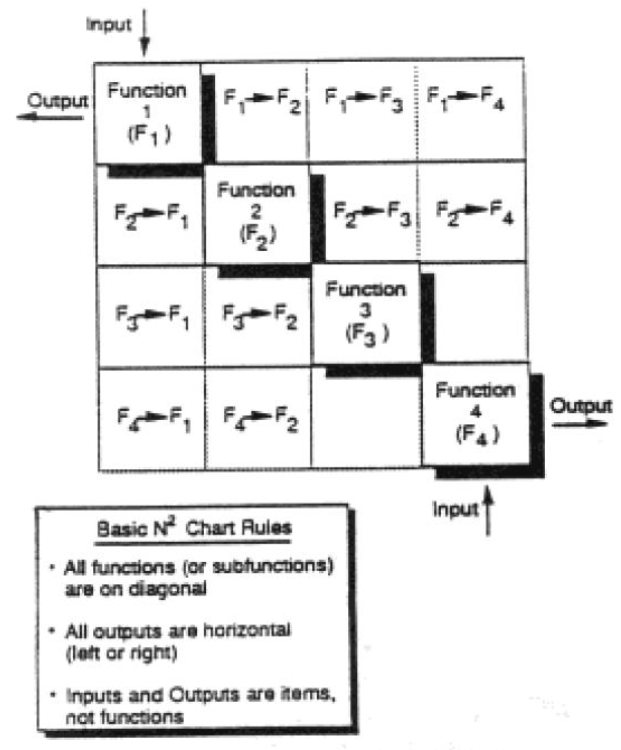
\includegraphics[scale=0.7]{img/NN}
	\caption{N2 modelio pavyzdys} % Antraštė įterpiama po paveikslėlio
	\label{img:mlp}
	\end{figure}



		Modeliavimas bus vykdomas Ad-hock principu, pasitelkiant praeities žinias arba tiesiog susėdus ekspertams ir bandant išsiaiškinti prindimą.
		Programų kūrimo proceso modeliavimą sudaro keturios dalys:
		\begin{enumerate}
			\item{Funkcinis modeliavimas - šiam modeliavimo žingsniui naudosime N2 lentelę(N2 Chart). Šioje diagramoje apibrėžiame funkcinias ir fizinias sąsajas tarp sistemos elementų }
			\item{Sistemos architektūra - šiame žingsnyje apibrėšime kaip sąveiką tarp skirtingų sistemos komponentų(duomenų bazių, servisų ir kitą) bei išorinių sistemų. Šiam modeliavimui bus pasitelkta UML komponentų diagramos.}
			\item{Verslo proceso modeliavimas - šiam modeliavimui bus naudojamos BPMN grafifai apibrėžentys verslo procesus. Sukurti procesai bus analizuojami, gerinami. Bus išskirtos verslo proceso dalys kurias galima automatizuoti.}
			\item{Įmonės modeliavimas - abstrakčiai sumodeliuojama kaip įmonės procesai įtakos tolimesnį programos vystymą. 
				Kokie procesų modeliai bus reikalingi sukurti pseudo kodui. Iš procesų modelių ir duomenų modelių kyla reikalavimai. }

		\end{enumerate}
	\subsection{Sistemos projektavimas}
	Projektuojant sistema siekiama patenkinti arba siekti išvardintas harakteristikas:
	\begin{itemize}
		\item{
			Intersuotų asmenų įvairovė - sistema turis patenkinti įvairių interesuotų asmenų norus ir poreikius, pavyzdžiui vadovai, savininkai, vartotojai ir valdytojai.
			%Kiekvienas interesuotas asmuo turi savo asmeninius interesuosus, kuriuos nori įvykdyti naudodamasis asmeninius interesuosus, kuriuos nori įvykdyti naudodamasis sistemą.
			%"Mėnuliukų technologijos" kompanijoje atidžiai ir glaustai bendraujama su interesuotais asmenimis tam kad tiksliai ir akivaizdžiai išsaiškinti interesuotais.
		}
		\item{Interesų atskyrimas - bandoma atskirti interesai taip, kad lengviau būtų realizuoti galutinėje sistemoje.  }
		\item{Remiamasi kokybės užtikrinimu - Bandoma taip pat siekti nefunkcinių reikalavimų užtikrinimu pavyzdžiui užtikrinti greitaveiką.}
	\end{itemize}
	% https://microservices.io
	\subsubsection{Mikroservisai}
	"Mėnuliukai technologijos" bando atskirti bendrą sistemą į daug mažesnių sistemų remdamasi dabartine populiaria mikroservisu architektūra.
	Kiekviena atskirta sistema turi būti kuo savarankiškesnė ir atlikti būtent vieną funkcionalumą, tačiau jį turės atlikti kuo efektyviau.
	Mikroservisai turi itin aiškiai apibrėžtas programų sąsajas bei dokumentaciją, kuri akivaizdžiai apibrėžia funkcionalumą.
	Taip užtikrinama, jog programų sistemos tikslingai atlieka reikalaujamus verslo siekius.

	\begin{figure}[H]
	\centering
	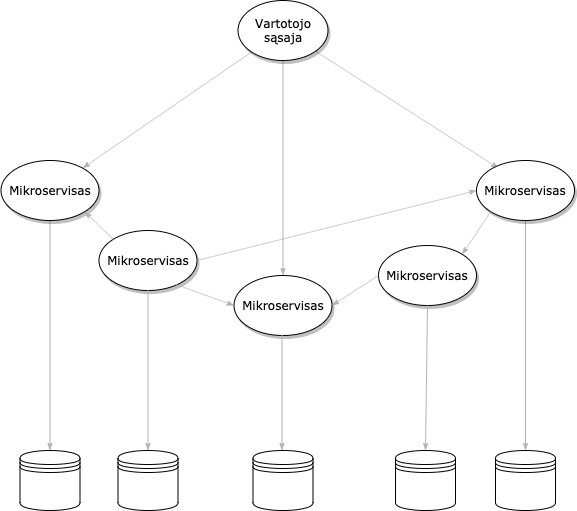
\includegraphics[scale=0.6]{img/micro.png}
	\caption{Mikroservisų architektūra}
	\label{img:mlp}
	\end{figure}
	Mikroservisų architektūros teikiami privalumai:
	\begin{itemize}
		\item{atskiros sistemos dalys yra lengviau prižiūrimos ir lengviau testuojamos}
		\item{silpna sistemos sąsajo - neglaudus sąryšis tarp komponentų bei programų leidžia daryti pakeitimus, kurie nepropaguoja per visą sistemą}
		\item{nepriklausomas servisų dalis galima atskirai diegti bei atlikti atnaujinimus nediegiant visos sistemos iš naujo}
		\item{Maži teamai prižiūri efektyviau sistemos, reikia mažiau komunikacijos}
		\item{Servisai kuriami pagal įmonės gebėjimus}
	\end{itemize}

	\subsection{Sistemos prototipavimas}
	Prototipavimo fazės rezultatas yra pirminė produkto versija, kuri jau detalesnė nei eskizai ar maketai. Prototipo fazėje dar galimaatrasti potencialias problemas ir, kadangi prototipas yra dar tik supaprastinta sistema, yra galimybė pakeisti produkto kūrimo kryptį be didelių nuostolių. Pavyzdžiui, pagal dizainą sukuriamas paprastas svetainės karkasas su kuriuo naudotojas gali sąveikauti: spausti mygtukus, įvesti duomenis į laukus. Jei sukurtas prototipas sėkmingas, investuojamas laikas ir pinigai į tolesnį produkto įgyvendinimą laikant prototipą jo pagrindu.
	\subsection{Sistemos įgyvendinimas}
	Šis žingsnis glaudžiai susijęs su prieš jį einančiomis fazėmis, jame vykdomas suprojektuotos sistemos dalies įgyvendinimas, kuris apima kodo rašymą, automatizuotų testų kūrimą, konfigūracijos pakeitimus ir duombazės kūrimą. Ši fazė įgyvendinama tik gerai išsiaiškinus ir susidokumentavus reikalavimus ir jau turint prototipą, kad kuriama programa atitiktų kliento lūkesčius ir reikalingų pakeitimų būtų mažiau.
	\subsection{Kokybės užtikrinimas}
	Kokybės užtikrinimas skirtingas kiekvienam projektui. Tuose projektuose, kuriuose kuriamoje sistemoje egzistuoja vartotojo sąsaja, atliekamas rankinis testavimas kartu su automatizuotu regresiniu testavimu. Į kokybės užtikrinimą yra įtraukiami ir programuotojai, kurie yra atsakingi už automatizuotų testų teisingumą. Testuotojai atsakingi už rankinį testavimą bei regresinių testų rezultatų apibendrinimą. Jeigu projektas yra iteracinis ir jau išleistas plačiam naudojimui, po sėkmingo testavimo kodas yra sudedamas į aukštesnę aplinką, kurioje yra papildomai pravaliduojamas prieš jį išleidžiant į produkciją.
	\subsection{Išleidimas}
	Išleidimo stadiją galima skaidyti į 2 skirtingus tipus - galimas naujas projekto išleidimas, kurio metu vartotojui pateikiama nauja sistema, kuri buvo tam tikrą laiką kuriama. Taip pat egzistuoja kitas variantas, kai yra veikianti sistema, kuri yra atnaujinama kas tam tikrą laiką (tai priklauso nuo sprinto ilgi). Išleidimo metu įmonėje yra vykdomi darbuotojų budėjimai, kad sistemai veikiant ne tiksliai pagal planą, sistemos trikdžiai būtų kuo greičiau pašalinti.
	\subsection{Palaikymas}
	Palaikymo procesui kuriamas palaikymo planas, susidedantis iš programos paruošimo, problemos identifikavimo bei produkto konfigūracijos valdymo. Problemos identifikavimas vykdomas tikrinant programos validumą, sukuriant problemos sprendinį bei išskiriant resursus modifikacijai įgyvendinti. Proceso patvirtinimas įgyvendinamas gavus patvirtinimą dėl kėtinamų įgyvendinti pakeitimų  iš užklausos autoriaus. Įmonė teikia dviejų tipų palaikymą: taisomąjį bei adaptacinį. Taisomasis palaikymas orientuotas į problemų, atrastų vartotojų arba vartotojų klaidų reportų analizės metu, taisymą. Adaptacinis palaikymas skirtas nūdienos standartų programose palaikymui. Įmonė laikosi „Boehm“ modelio, kuris pasižymi atitinkamai pakeitimų pasiūlymu, patvirtinimu bei įgyvendinimu. *Boehm's model graph will insert later* 

	\subsection{Balius/Post-mortem}
	Procesas užbaigiamas komandos bei prie projekto prisidėjusių žmonių švente, kurioje aptariamas bei įvertinamas proceso pasisekimas ir daromos išvados.

\sectionnonum{Rezultatai ir išvados}



\end{document}
